\documentclass[12pt, oneside]{article}

\usepackage[letterpaper, scale=0.89, centering]{geometry}
\usepackage{fancyhdr}
\setlength{\parindent}{0em}
\setlength{\parskip}{1em}

\pagestyle{fancy}
\fancyhf{}
\renewcommand{\headrulewidth}{0pt}
\rfoot{\href{https://creativecommons.org/licenses/by-nc-sa/2.0/}{CC BY-NC-SA 2.0} Version \today~(\thepage)}

\usepackage{amssymb,amsmath,pifont,amsfonts,comment,enumerate,enumitem}
\usepackage{currfile,xstring,hyperref,tabularx,graphicx,wasysym}
\usepackage[labelformat=empty]{caption}
\usepackage[dvipsnames,table]{xcolor}
\usepackage{multicol,multirow,array,listings,tabularx,lastpage,textcomp,booktabs}

\lstnewenvironment{algorithm}[1][] {   
    \lstset{ mathescape=true,
        frame=tB,
        numbers=left, 
        numberstyle=\tiny,
        basicstyle=\rmfamily\scriptsize, 
        keywordstyle=\color{black}\bfseries,
        keywords={,procedure, div, for, to, input, output, return, datatype, function, in, if, else, foreach, while, begin, end, }
        numbers=left,
        xleftmargin=.04\textwidth,
        #1
    }
}
{}
\lstnewenvironment{java}[1][]
{   
    \lstset{
        language=java,
        mathescape=true,
        frame=tB,
        numbers=left, 
        numberstyle=\tiny,
        basicstyle=\ttfamily\scriptsize, 
        keywordstyle=\color{black}\bfseries,
        keywords={, int, double, for, return, if, else, while, }
        numbers=left,
        xleftmargin=.04\textwidth,
        #1
    }
}
{}

\newcommand\abs[1]{\lvert~#1~\rvert}
\newcommand{\st}{\mid}

\newcommand{\A}[0]{\texttt{A}}
\newcommand{\C}[0]{\texttt{C}}
\newcommand{\G}[0]{\texttt{G}}
\newcommand{\U}[0]{\texttt{U}}

\newcommand{\cmark}{\ding{51}}
\newcommand{\xmark}{\ding{55}}

 
\begin{document}
\begin{flushright}
    \StrBefore{\currfilename}{.}
\end{flushright} 

\vspace{-1cm}
\section*{Before we start}
If you or someone you know is suffering from food and/or housing insecurities 
there are UCSD resources here to help:

Basic Needs Office: \href{https://basicneeds.ucsd.edu/}{https://basicneeds.ucsd.edu/}

Triton Food Pantry (in the old Student Center)
is free and anonymous, and includes produce: 

\href{https://www.facebook.com/tritonfoodpantry/}{https://www.facebook.com/tritonfoodpantry/}

Mutual Aid UCSD: \href{https://mutualaiducsd.wordpress.com/}{https://mutualaiducsd.wordpress.com/}

If you find yourself in an uncomfortable situation, ask for help. 
We are committed to upholding University policies regarding nondiscrimination, sexual violence and sexual harassment.

Counseling and Psychological Services (CAPS) at 858 5343755 or \href{http://caps.ucsd.edu}{http://caps.ucsd.edu}


OPHD at (858) 534-8298, ophd@ucsd.edu , \href{http://ophd.ucsd.edu}{http://ophd.ucsd.edu}. 
CARE at Sexual Assault Resource Center at 858 5345793 sarc@ucsd.edu \href{http://care.ucsd.edu}{http://care.ucsd.edu}

\vspace{-0.5cm}
\subsection*{Pandemic resilient instruction}
{\small
Spring 2022 feels like the first quarter post-pandemic. We were all kind of blindsided with Omicron last quarter and so we should all be cautious about what we expect to happen. We will keep a close eye on university policies and will inform the class whenever there is a change to our class policy.

I will be giving lectures in-person. I will also offer remote support throughout the quarter. Throughout the quarter, the "in-person" lectures will be live-streamed through zoom and recorded via "podcast.ucsd.edu". The exams will be offered "in-person" or "remote" and each student can choose which type of exam they prefer. This way we can be ready for whatever lies ahead and also give students the option of how they want to interact with the class.

First and foremost is the health and safety of everyone.  Please do not come to class if you are sick or even think you might be sick.  It is likely that the university will be requiring masks and "symptom screeners" and/or "covid tests". We expect all students to follow the rules. With all of this in mind, we encourage all students to come to class when they can, but will also provide as much of the class materials as we can in a remotely viewable format. The lectures are designed to engage students in real time with opportunities for questions and discussions between instructor and students and also between students and other students.   We will also have some ways for students who participate remotely to engage in discussions with the instructors and other students, but cannot guarantee the full experience for remote students. 

(Personal note: Last quarter (Winter 2022), we started online and returned to campus mid-quarter. After that, I ran my classes in a similar way. I am hopeful to expect that Spring quarter will be fully in person but I am a bit wary. For that reason, I have decided to continue offering the remote option for Spring 2022 mainly due to the fact that I do not know what the future will hold. There are many things about teaching remotely that I found to be great and I will try to incorporate some lessons learned from my remote teaching experience. I am excited and hopeful to teach a quarter fully "in-person". I will try my best to bring a classroom experience that is the best of both worlds.
-Miles Jones) }




\newpage
Welcome to CSE 20: Discrete Math for Computer Science in Fall 2021! 

\section*{Themes and applications for CSE 20}
\begin{itemize}
\item {\bf Technical skepticism}: Know, select and apply appropriate computing knowledge and problem-solving techniques. 
Reason about computation and systems. 
Use mathematical techniques to solve problems. 
Determine appropriate conceptual tools to apply to new situations. 
Know when tools do not apply and try different approaches. 
Critically analyze and evaluate candidate solutions.
\item {\bf Multiple representations}: Understand, guide, shape impact of computing on society/the world. 
Connect the role of Theory CS classes to other applications (in undergraduate CS curriculum and beyond). 
Model problems using appropriate mathematical concepts.
Clearly and unambiguously communicate computational ideas using appropriate formalism. 
Translate across levels of abstraction.
\end{itemize}

{\bf Applications}: Numbers (how to represent them and use them in Computer Science), 
Recommendation systems and their roots in machine learning (with applications like Netflix),
``Under the hood" of computers (circuits, pixel color representation, data structures),
Codes and information (secret message sharing and error correction),
Bioinformatics algorithms and genomics (DNA and RNA).

\section*{Introductions}
Class website: There is a link to a class website from my homepage: \href{https://cseweb.ucsd.edu/~mej016/}{https://cseweb.ucsd.edu/\~{}mej016/}

I am also using Canvas as a website.

(I am transitioning from Canvas to a new resource that the department has been developing. It has been initiated by Mia Minnes and Joe Politz with help from Aiko Coanaya and Akanksha Pandey.)



{\bf Pro-tip}: you can use MATH109 to replace CSE20 for prerequisites and other requirements.

Instructor: Miles Jones

Our team: Five TAs and 8 tutors + all of you




On a typical week: {\bf TuTh} Lectures + review quizzes, {\bf W} HW due, {\bf M} Discussion, office hours, Piazza. 
Tests and Midterms see the content calendar.





\newpage
\section*{Tuesday March 29}


What data should we encode about each Netflix account holder to help us make effective recommendations?

\vfill
\vfill

In machine learning, clustering can be used to group similar data for prediction and recommendation.  For example,
each Netflix user's viewing history can be represented as a $n$-tuple indicating their preferences about
movies in the database, where $n$ is the number of movies in the database.  People with similar tastes in movies can then be clustered to provide recommendations
of movies for one another.  Mathematically, clustering is based on a notion of distance between pairs of $n$-tuples.
 

In the table  below,  each row represents a user's ratings of movies: 
\cmark~(check) indicates the person liked the movie, \xmark~(x)
that they didn't, and $\bullet$ (dot) that they didn't rate it one way or 
another (neutral rating or didn't watch). Can encode
these ratings numerically with $1$ for \cmark~(check), $-1$ for \xmark~(x), 
and $0$ for $\bullet$ (dot).

\begin{center}
\begin{tabular}{c|ccc||c}
Person & Fyre & Frozen II & Picard & Ratings written as a  $3$-tuple\\
\hline
$P_1$     & \xmark & $\bullet$ & \cmark & \phantom{$(-1, 0, 1)$} \\
$P_2$     & \cmark & \cmark & \xmark & \phantom{$(1, 1, -1)$} \\
$P_3$     & \cmark & \cmark & \cmark & \phantom{$(1, 1, 1)$} \\
$P_4$     & $\bullet$ & \xmark & \cmark &  \\
\end{tabular}
\end{center} 
{\bf Conclusion}: Modeling involves choosing data types to represent and organize data

\newpage

\subsection*{Discrete Math vs Continuous Math}

\begin{multicols}{2}
  {\bf Continuous Math}\\
  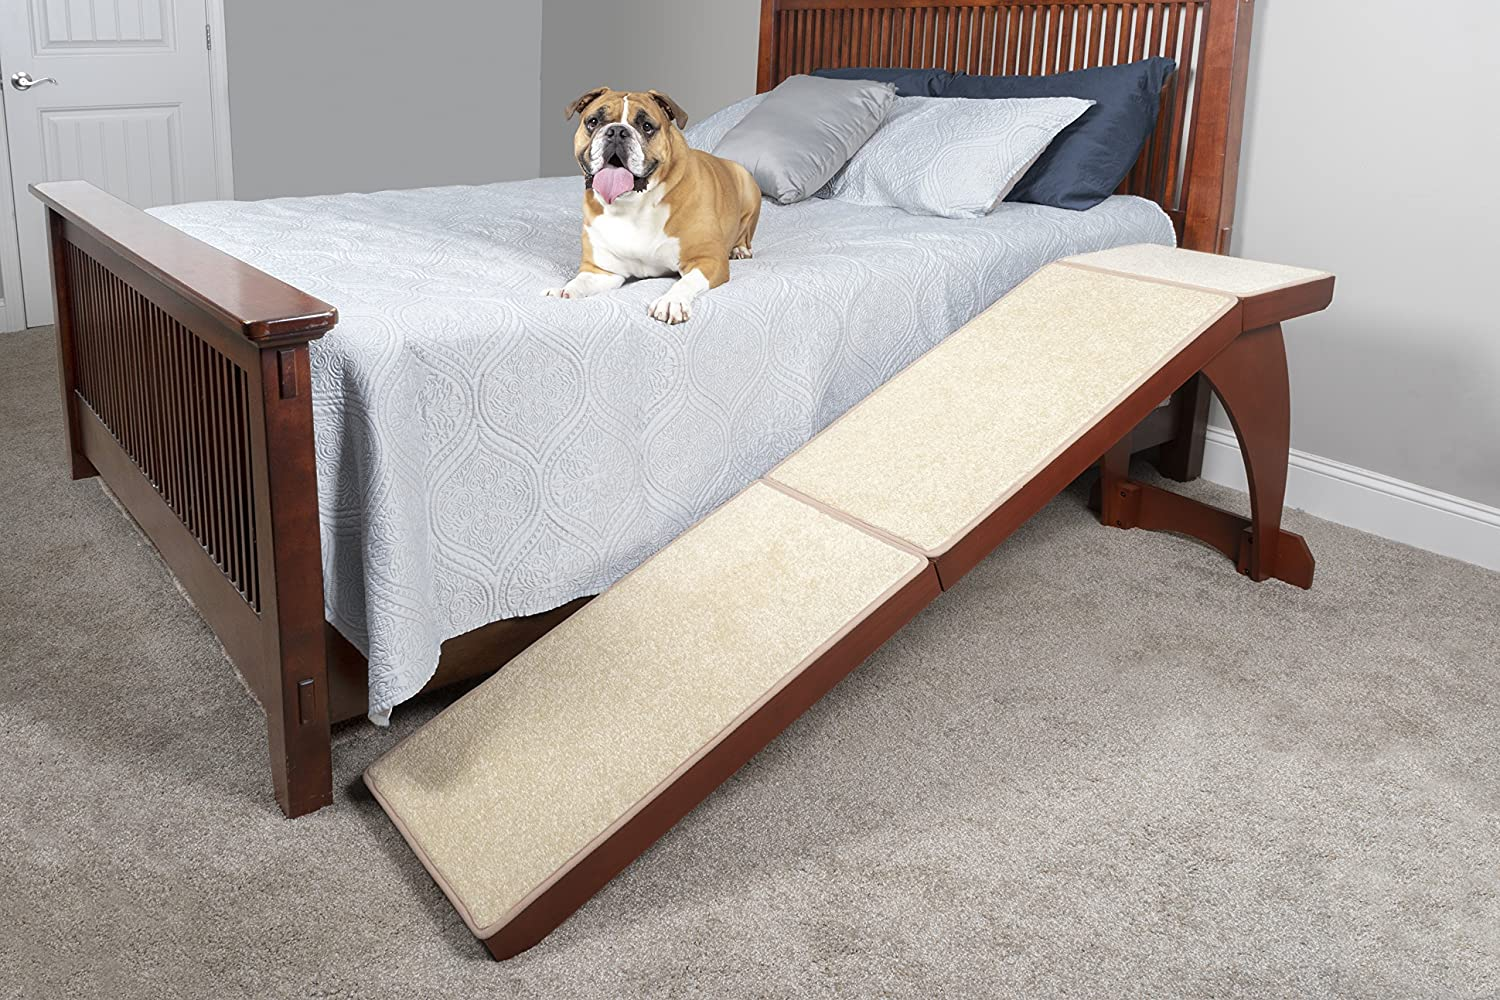
\includegraphics[scale=0.1]{../../resources/images/dog_ramp.jpg} 
  \href{https://www.google.com/imgres?imgurl=httpsContinuous math is the study of the \emph{real number line}\\
  What are some subjects that would be considered as continuous math?
  
  {\bf Discrete Math}\\
  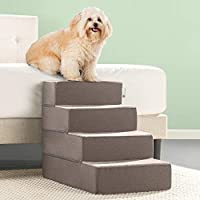
\includegraphics[scale=0.5]{../../resources/images/dog_stairs.jpg}
   \href{https://www.google.com/imgres?imgurl=httpsDiscrete math deals with distinct objects (like the integers.)\\
  What are some subjects that would be considered as discrete math?
  
\end{multicols}
\vfill

{\bf Math and computer science.}

What are some ways that math is used in computer science?

\vfill



\newpage


\subsection*{Notation and prerequisites}

\begin{center}
\begin{tabular}{|llp{9.8cm}|}
\hline
{\bf Term} & {\bf Notation Example(s)} & {\bf We say in English \ldots } \\
\hline
sequence & $x_1, \ldots, x_n$ & A sequence $x_1$ to $x_n$ \\
summation & $\sum_{i=1}^n x_i$ or $\displaystyle{\sum_{i=1}^n x_i}$ & The sum of the terms of the sequence $x_1$ to $x_n$ \\
&&\\
all reals & $\mathbb{R}$ & The (set of all) real numbers (numbers on the number line)\\
all integers & $\mathbb{Z}$ & The (set of all) integers (whole numbers including negatives, zero, and positives) \\
all positive integers & $\mathbb{Z}^+$ & The (set of all) strictly positive integers \\
all natural numbers & $\mathbb{N}$ or $\mathbb{Z}^{\geq 0}$ & The (set of all) natural numbers. {\bf Note}: we use the convention that $0$ is a natural number. \\
&&\\
piecewise rule definition & $f(x) = \begin{cases} x & \text{if~}x \geq 0 \\ -x & \text{if~}x<0\end{cases}$ &
Define $f$ of $x$ to be $x$ when $x$ is nonnegative and to be $-x$ when $x$ is negative\\
function application & $f(7)$ & $f$ of $7$ {\bf or} $f$ applied to $7$ {\bf or} the image of $7$ under $f$\\
                     & $f(z)$ & $f$ of $z$ {\bf or} $f$ applied to $z$ {\bf or} the image of $z$ under $f$\\
                     & $f(g(z))$ & $f$ of $g$ of $z$ {\bf or} $f$ applied to the result of $g$ applied to $z$ \\
&&\\
absolute value & $\lvert -3 \rvert$ & The absolute value of $-3$ \\
square root & $\sqrt{9}$ & The non-negative square root of $9$ \\
&&\\


\hline
\end{tabular}
\end{center}

{\bf Mathematical object and data types}

A mathematical object is any abstract object arising in mathematics.

What are some examples of mathematical objects?

\vfill

Computers encode mathematical objects into data types. What are some examples of data types?

\vfill

\newpage

\subsection*{Data Types: sets, $n$-tuples, and strings}


\begin{center}
    \begin{tabular}{p{4.6in}p{2.6in}}
    {\bf  Term} & {\bf Examples}:\\
    &  (add additional examples from class)\\
    \hline 
    {\bf set} \newline
    unordered collection of elements & $7 \in \{43, 7, 9 \}$ \qquad $2 \notin \{43, 7, 9 \}$ \\
    {\it repetition doesn't matter} & \\
    {\it Equal sets agree on membership of all elements}& \\
    \hline
    {\bf $n$-tuple} (also called an {\bf $n$-dimensional vector}) \newline
    ordered sequence of entries with $n$ ``slots" ($n >0$) & \\
    {\it repetition matters, fixed length} &\\
    {\it Equal $n$-tuples have corresponding entries equal}& \\
    \hline
    {\bf string} \newline
    ordered finite sequence of elements each from specified
    set & \\
    {\it repetition matters, arbitrary finite length} &\\
    {\it Equal strings have same length and corresponding characters equal}
    \end{tabular}
\end{center}

{\it Special cases}: 

When $n=2$, the 2-tuple is called an {\bf ordered pair}.

A string of length $0$ is called the {\bf empty string} and is denoted $\lambda$.

A set with no elements is called the {\bf empty set} and is denoted $\{\}$ or $\emptyset$. 

\subsection*{Sets}

A set is an unordered collection of \emph{elements}.

Recall that the empty set (denoted $\emptyset$ or $\{~\}$) is the set without any elements.

{\it To define sets:}

To define a set using {\bf roster method}, explicitly list its elements using \emph{curly braces}. That is,
start with $\{$ then list elements of 
the set separated by commas and close with $\}$.

To define a set using {\bf set builder definition}, either form 
``The set of all $x$ from the universe $U$ such that $x$ is ..." by writing
\[\{x \in U \mid ...x... \}\]
or form ``the collection of all outputs of some operation when the input ranges over the universe $U$"
by writing
\[\{ ...x... \mid x\in U \}\]

We use the symbol $\in$ as ``is an element of'' to indicate membership in a set.\\

\newpage

{\bf Example sets}: For each of the following, identify whether it's defined using the roster method
or set builder notation and give an example element.
\begin{itemize}
    \item[]$\{ -1, 1\}$\\
    \item[]$\{0, 0 \}$\\
    \item[]$\{-1, 0, 1 \}$\\
    \item[]$\{(x,x,x) \mid x \in \{-1,0,1\} \}$\\
    \item[]$\{ \}$\\
    \item[]$\{ x \in \mathbb{Z} \mid x \geq 0 \}$\\
    \item[]$\{ x \in \mathbb{Z}  \mid x > 0 \}$\\
    \item[]$\{\A,\C,\U,\G\}$ \\
    \item[]$\{\A\U\G, \U\A\G, \U\G\A, \U\A\A \}$
\end{itemize}

\subsection*{$n$-tuples}

An $n$-tuple is a sequences of $n$ \emph{entries}.

\emph{To define $n$-tuples}

To define $n$-tuples, list the entries separated by commas and enclosed by parentheses.

{\bf Example $n$-tuples}: For each of the following $n$-tuple, come up with where it might come from. For example, $(88, 79, 100, 90, 68, 81,90)$ may be the grades a particular student will get for homeworks 1-7.

\begin{itemize}
    \item[]$(1,2.22, -0.8)$\\
    \item[]$(-1,-1,0,1,0,-1,0,0)$\\
    \item[]$(CSE20, CSE21, CSE101, CSE105)$\\
    \item[]$(MILES,JONES,A000000,MUIR,91.86,A-)$
\end{itemize}


\newpage

\subsection*{strings (over a finite alphabet)}

A string over a finite alphabet is a finite sequence of \emph{characters} or \emph{symbols}.

Recall that the \emph{empty string}, (usually denoted $\lambda$) is the string without any characters.

The characters you are allowed to use come from a finite set called an \emph{alphabet}.

\emph{To define strings:}

Usually, a string is given as a list of characters without any punctuation. In some cases, we will use the symbol ``$\circ$" as a delimiter. For example, if the alphabet is $\{\A,\C,\U,\G\}$, then consider the string $\A\A\A\U\A$. It could also be written as $\A\circ\A\circ\A\circ\U\circ\A$.

\emph{string concatenation}

String concatenation of strings $x$ and $y$, denoted $xy$ or $x\circ y$ is the result of ``gluing together" the strings $x$ first then $y$. For example: $\A\U\A\A\circ \G\G\C=\A\U\A\A\G\G\C$.

{\bf Pro-tip}: the meaning of writing one element next to another like $xy$ depends on the data-types of $x$ and 
$y$. When $x$ and $y$ are strings, the convention is that $xy$ is the result of string concatenation. 
When $x$ and $y$ are numbers, the convention is that $xy$ is the result of multiplication. This is 
(one of the many reasons) why is it very important to declare the data-type of variables before we use them.


{\bf Example strings}: For each example, come up with an appropriate alphabet:
\begin{itemize}
    \item[]$MATHEMATICS$\\
    \item[]$A00000000$\\
    \item[]$2598960$\\
    \item[]$\C\C\A\C\U\G\C\C\A$\\
    \item[]$\lambda$\\
    \item[]$9500~Gilman~Dr.$\\
    \item[]$11100010101101000111111011111$\\
    \item[]$mej016@eng.ucsd.edu$ \\
    \item[]$F96A4B0B$
\end{itemize}


\end{document}